\documentclass[UTF8,a4paper,12pt]{ctexart}

\usepackage{amsmath,amssymb}
\usepackage{booktabs}
\usepackage{array}
\usepackage{float}
\usepackage{geometry}
\usepackage{graphicx}
\usepackage{hyperref}
\usepackage{xcolor}
\usepackage{listings}
\usepackage{fancyhdr}

\geometry{left=2.6cm,right=2.6cm,top=2.6cm,bottom=2.6cm}
\graphicspath{{assets/}}
\hypersetup{
  colorlinks=true,
  linkcolor=black,
  urlcolor=black,
  citecolor=black,
  allcolors=black
}

\lstset{
  basicstyle=\ttfamily\small,
  breaklines=true,
  columns=fullflexible,
  frame=single,
  rulecolor=\color{black!20},
  backgroundcolor=\color{black!3}
}

\pagestyle{fancy}
\fancyhf{}
\cfoot{\thepage}
\renewcommand{\headrulewidth}{0pt}
\renewcommand{\footrulewidth}{0pt}
\fancypagestyle{plain}{
  \fancyhf{}
  \cfoot{\thepage}
  \renewcommand{\headrulewidth}{0pt}
  \renewcommand{\footrulewidth}{0pt}
}

\ctexset{
  section = {
    number = \chinese{section}、,
    aftername = {},
    tocline = {\csname CTEXthe#1\endcsname#2}
  },
  subsection = {
    number = (\chinese{subsection}),
    aftername = {\quad}
  }
}

\title{\heiti 含噪图像去噪与清晰图像恢复实时演示系统}
\author{第 11 小组\quad 智文静，奚奕萱，汪语菲，黄冠杰}
\date{\today}

\begin{document}

\pagenumbering{Roman}
\pagestyle{fancy}
\maketitle
\thispagestyle{fancy}

\begin{abstract}
本项目构建了一个可实时上传、实时加噪、实时计算并可下载结果的图像去噪演示系统。系统围绕含噪图像恢复这一典型二维信号处理问题，分别实现了空域滤波、频域滤波、保边滤波、非局部均值去噪和后处理锐化。基础部分支持高斯噪声、椒盐噪声、混合噪声和横向周期噪声，并对均值滤波、中值滤波、高斯低通、巴特沃斯低通、多组径向 Band-Stop、成对陷波带阻滤波器进行对比。进阶部分实现双边滤波与非局部均值（NLM），讨论参数对去噪和保边的影响。系统还提供参考指标、无参考质量评价、频谱分析、贝叶斯优化调参、USM 非锐化掩膜和一键导出功能。
\end{abstract}

\clearpage
\tableofcontents
\clearpage
\pagenumbering{arabic}
\pagestyle{fancy}

\section{引言}

图像可以看作定义在二维空间上的离散信号。在实际采集、传输和存储过程中，图像常受到传感器热噪声、量化误差、传输脉冲干扰或周期性设备干扰的影响，从而产生高斯噪声、椒盐噪声、周期条纹等失真。图像去噪的目标是在抑制噪声的同时尽可能保留边缘、纹理和结构信息。

本项目选择“含噪图像去噪与清晰图像恢复”作为主题，原因在于它能够自然连接信号与系统课程中的卷积、滤波、频域分析和系统响应等核心概念。空域滤波体现二维卷积与邻域统计，频域滤波体现二维离散傅里叶变换（DFT）和频率响应设计，双边滤波与 NLM 则进一步说明线性滤波在边缘保持方面的局限\cite{gonzalez2018digital,tomasi1998bilateral,buades2005nlm}。

本系统要求用户在界面中上传任意图片，随后选择噪声类型、配置滤波参数、实时运行去噪算法并观察结果。

\section{任务目标与系统设计}

\subsection{任务目标}

根据课程任务要求，本项目的功能目标可以分为基础、进阶和挑战三个层次：

\begin{enumerate}
  \item 基础任务：对含不同噪声的图像分别实现均值滤波、中值滤波等空域滤波，观察并对比效果；对含噪图像做 DFT 频谱分析，设计合适的频域滤波器并与空域方法进行比较。
  \item 进阶任务：实现双边滤波，分析空间标准差和灰度标准差对“去噪”与“保边”的影响。
  \item 挑战任务：针对混合噪声和真实受损图像场景，引入 NLM、无参考质量评价、参数自动调优和 USM 后处理锐化，使程序具备更完整的演示价值。
\end{enumerate}

\subsection{系统交互流程}

系统采用 Streamlit 构建，运行后用户首先上传图像或选择演示预设。程序将像素归一化到 $[0,1]$，再根据侧边栏参数生成当前含噪输入，最后对用户选定的方法逐一计算输出。界面顶部提供五个观察视图：图像、频谱、灰度直方图、边缘和后处理锐化。

\begin{figure}[H]
  \centering
  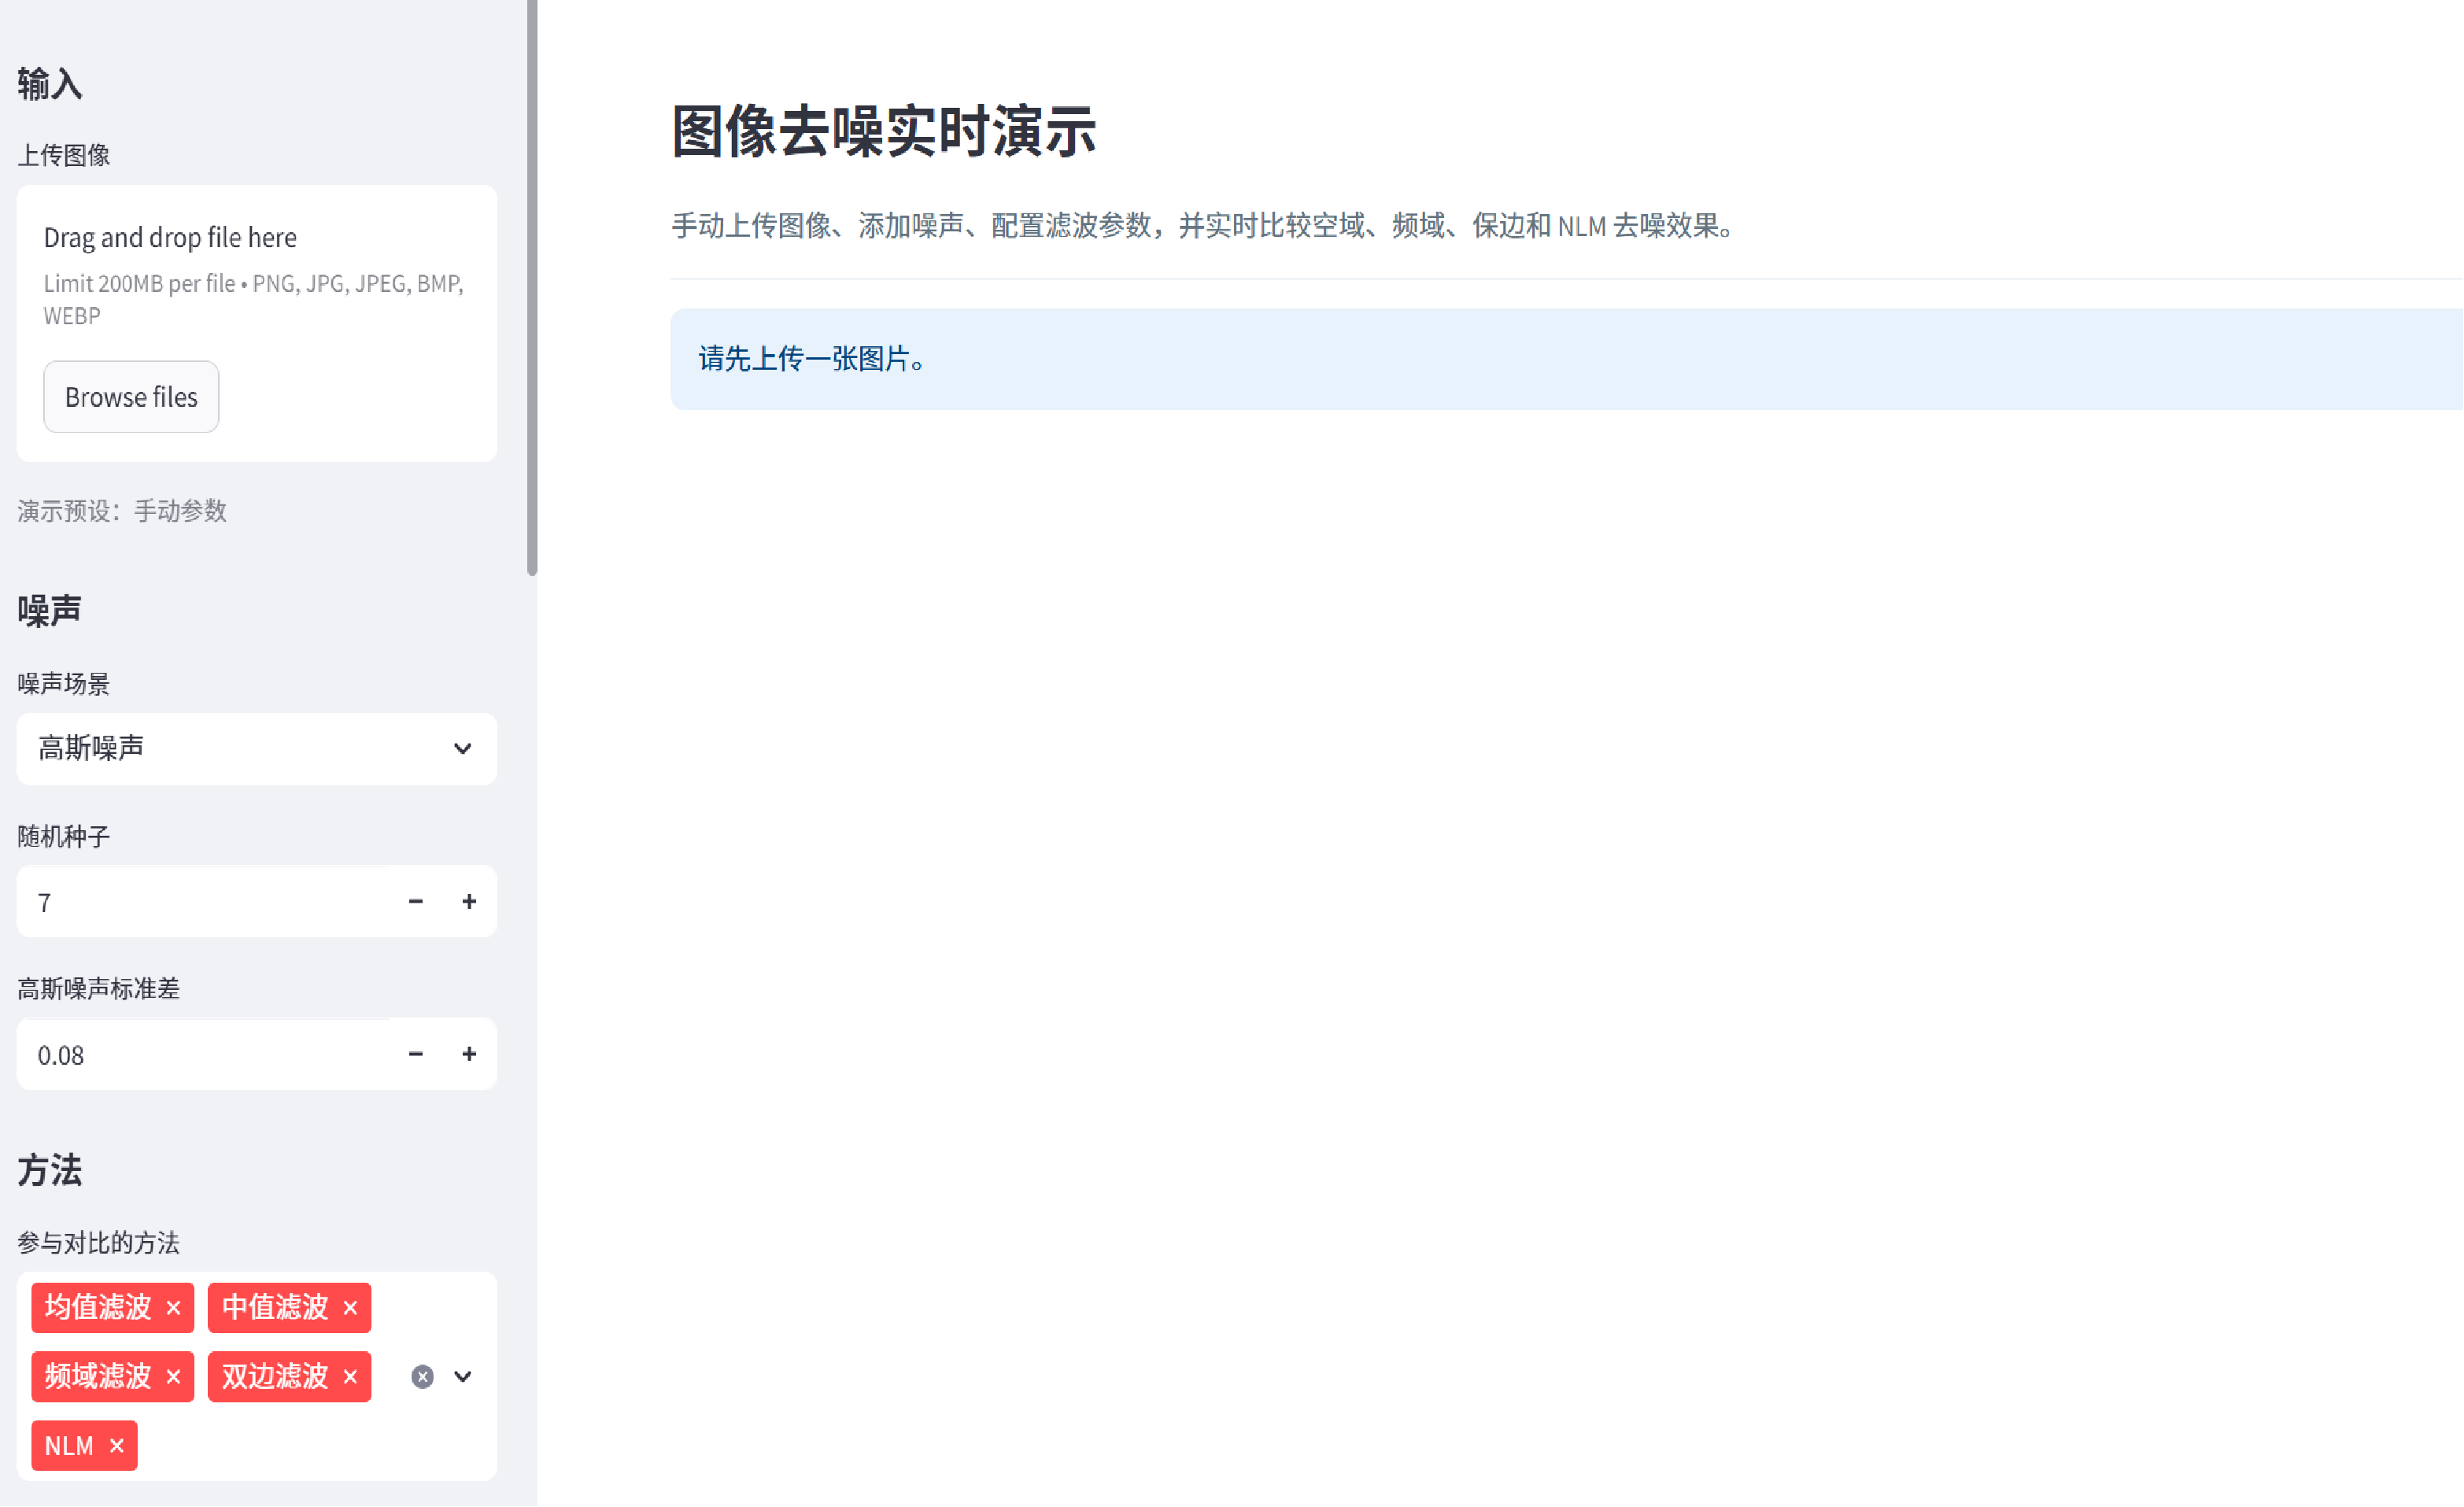
\includegraphics[width=0.92\linewidth]{new_image/系统演示图.png}
  \caption{实时演示系统界面}
  \label{fig:system-ui}
\end{figure}

系统不仅展示滤波后的图像，还显示原图频谱、含噪图频谱、频域滤波后频谱、频域响应、灰度直方图和边缘图。所有关键图像和表格均可下载，并支持一键导出包含图像、CSV 指标、频域响应和当前参数 JSON 的压缩包，方便课后复现实验。

\subsection{代码结构}

项目将算法实现和界面逻辑分离。核心目录 \texttt{denoise\_lab} 中，\texttt{noise.py} 负责噪声生成，\texttt{spatial.py} 负责均值与中值滤波，\texttt{frequency.py} 负责频域响应和频域滤波，\texttt{advanced.py} 负责双边滤波与 NLM，\texttt{analysis.py} 负责频谱、边缘、直方图和参考指标，\texttt{auto\_tune.py} 负责参数搜索，\texttt{no\_reference.py} 负责无参考评价，\texttt{sharpening.py} 负责 USM 后处理。部分图像基础算子复用 scikit-image 与 SciPy 的成熟实现，以保证课程演示重点集中在方法对比和参数解释上\cite{skimage}。

\begin{lstlisting}[language=Python,caption={项目主要模块划分}]
app.py                         # Streamlit 界面和交互逻辑
denoise_lab/noise.py           # 高斯、椒盐、混合、周期噪声
denoise_lab/spatial.py         # 均值滤波、中值滤波
denoise_lab/frequency.py       # 频域滤波器响应与滤波
denoise_lab/spectrum_advisor.py# 频谱分析和参数建议
denoise_lab/advanced.py        # 双边滤波、NLM
denoise_lab/analysis.py        # 频谱、直方图、边缘、指标
denoise_lab/auto_tune.py       # BO 自动调参
denoise_lab/sharpening.py      # USM 非锐化掩膜
\end{lstlisting}

为了保证报告内容能够对应到实际程序，下面在各算法章节穿插核心代码摘录。代码并非伪代码，而是项目模块中的主要实现逻辑。界面层只负责收集参数和展示结果，真正的图像处理函数保持为可复用、可测试的 NumPy 数组输入输出形式。

\begin{lstlisting}[language=Python,caption={噪声生成模块的核心逻辑}]
def add_noise(image, noise_type, gaussian_sigma, sp_amount,
              periodic_strength, periodic_frequency, seed):
    rng = np.random.default_rng(seed)
    result = np.clip(image, 0.0, 1.0)

    if noise_type in {"高斯噪声", "混合噪声"}:
        result = util.random_noise(
            result, mode="gaussian",
            mean=0.0, var=float(gaussian_sigma) ** 2, rng=rng)

    if noise_type in {"椒盐噪声", "混合噪声"}:
        result = util.random_noise(
            result, mode="s&p", amount=float(sp_amount), rng=rng)

    if noise_type == "周期噪声":
        h = result.shape[0]
        yy = np.arange(h)[:, None]
        wave = np.sin(2 * np.pi * int(periodic_frequency) * yy / max(h, 1))
        result = result + float(periodic_strength) * wave[..., None]

    return np.clip(result, 0.0, 1.0)
\end{lstlisting}

\section{工程实现细节}

\subsection{图像输入与数据规范}

为了保证不同算法之间的比较公平，系统在读入图像后统一转换为浮点数组，并把像素值裁剪到 $[0,1]$。若用户上传的是彩色图像，则大多数滤波算法保持 RGB 三通道处理；需要显示频谱、直方图、边缘图或无参考评价时，程序再临时转换为灰度图。这种设计避免了两个问题：一是避免在算法处理阶段过早丢失颜色信息，二是保证所有指标计算都使用一致的动态范围。

系统区分两种输入语义。第一种是“上传原清晰图”，程序会根据用户选择实时添加噪声，此时原图就是参考图，可以计算 MSE、PSNR 和 SSIM，也可以用这些指标进行 BO 自动调参。第二种是“上传图像已含噪”，程序不再叠加额外噪声，此时不存在干净参考图，参考指标关闭，自动调参改用 NIQE-like 无参考评价。这个区分直接影响指标口径，因此在界面侧用噪声场景“无：上传图像已含噪”显式表达。

\begin{table}[H]
\centering
\caption{两类输入场景的数据口径}
\begin{tabular}{p{0.24\linewidth}p{0.31\linewidth}p{0.31\linewidth}}
\toprule
输入场景 & 参考图与指标 & 自动调参口径 \\
\midrule
上传清晰图并加噪 & 原上传图作为参考图，计算 MSE、PSNR、SSIM & 最大化 $J=\operatorname{SSIM}+\operatorname{PSNR}/60-\min(25\operatorname{MSE},2)$ \\
上传图像已含噪 & 无干净参考图，不显示参考指标 & 最小化 NIQE-like 无参考分数，结果仅作为建议 \\
\bottomrule
\end{tabular}
\end{table}

\subsection{实时计算流程}

每次侧边栏参数发生变化，Streamlit 会重新执行脚本。系统利用这一机制把“上传图像、生成含噪输入、执行滤波、展示结果”组织成确定性的流水线。随机噪声由用户输入的随机种子控制，因此同一张图、同一组参数和同一个种子可以稳定复现实验结果。滤波方法以列表形式选择，程序逐个运行并把输出保存到字典中，后续的图像页、频谱页、直方图页和边缘页都从同一份输出字典读取，避免不同页面重复计算导致结果不一致。

实时演示时，推荐先只选择一种方法观察单一参数的影响，再逐步增加对比方法。例如高斯噪声下先比较均值滤波、双边滤波和 NLM；椒盐噪声下先比较中值滤波与均值滤波；周期噪声下先切到频谱页观察异常亮点，再回到参数区手动输入陷波点。这样可以保证演示过程和算法逻辑同步推进，而不是只展示最终结果。

\begin{table}[H]
\centering
\caption{系统实时演示流程}
\begin{tabular}{p{0.16\linewidth}p{0.35\linewidth}p{0.35\linewidth}}
\toprule
阶段 & 操作 & 说明重点 \\
\midrule
上传图像 & 选择纹理、边缘较明显的图片 & 便于观察模糊、保边和频谱变化 \\
添加噪声 & 依次选择高斯、椒盐、周期或混合噪声 & 对应不同噪声模型与频域特征 \\
选择方法 & 先单方法，再多方法对比 & 明确每种滤波器适用条件 \\
调整参数 & 修改核大小、截止频率、陷波点和保边参数 & 展示参数变化对结果的影响 \\
导出结果 & 下载图像、CSV 指标和参数 JSON & 保证报告结果可复现 \\
\bottomrule
\end{tabular}
\end{table}

\subsection{频谱页与参数设计}

频谱页的作用不是单纯展示一张图，而是帮助用户从频域角度解释滤波器为什么这样设计。系统展示原图频谱、含噪图频谱、频域滤波后频谱和滤波器响应。对于周期噪声，用户应寻找远离频谱中心且关于中心成对出现的亮点；对于径向异常能量，用户应关注某个半径附近是否出现环状增强；对于高频随机噪声，用户应观察频谱外圈是否整体变亮。

项目中还实现了沿 $x$ 轴和 $y$ 轴的一维频谱剖面。其核心思路是分别沿图像水平方向和竖直方向做一维 FFT，再取中心行或中心列的幅度谱。这与二维频谱图互补：二维频谱适合直观看亮点、亮线和环状结构，一维剖面适合定量估计异常峰相对中心的频率偏移。

\begin{lstlisting}[language=Python,caption={轴向频谱剖面的计算方式}]
def axis_spectra(image: np.ndarray) -> dict[str, np.ndarray]:
    gray = to_gray(image)
    h, w = gray.shape
    spectrum_x = np.fft.fftshift(np.fft.fft(gray, axis=1), axes=1)
    spectrum_y = np.fft.fftshift(np.fft.fft(gray, axis=0), axes=0)
    profile_x = np.log1p(np.abs(spectrum_x[h // 2, :]))
    profile_y = np.log1p(np.abs(spectrum_y[:, w // 2]))
    return {
        "x_frequency": np.linspace(-0.5, 0.5, w) * w,
        "x_profile": profile_x,
        "y_frequency": np.linspace(-0.5, 0.5, h) * h,
        "y_profile": profile_y,
    }
\end{lstlisting}

在手动设置陷波点时，应先记录图像尺寸与频谱中心，再由亮点坐标减去中心坐标得到 $(u_k,v_k)$。若亮点为 $(u_c+\Delta u,v_c+\Delta v)$，则另一侧通常在 $(u_c-\Delta u,v_c-\Delta v)$。本项目的成对陷波带阻参数直接使用相对偏移，因此用户只需输入一组 $(\Delta u,\Delta v)$，系统会自动生成正负对称的抑制区域。若有多组亮点，则添加多组陷波参数；若异常能量呈一条连续亮线，单点陷波通常不够，需要通过多组陷波点近似覆盖亮线。

\subsection{下载与复现设计}

报告和课堂展示中的实验结论必须能够复现，因此系统提供单图下载和总 ZIP 下载两类方式。单图下载适合把当前视图中的某一张结果保存到 PPT；总 ZIP 下载则面向完整实验记录，包含原图或上传图、当前含噪输入、含噪图频谱、所有滤波结果、参考指标 CSV、灰度直方图 CSV、频域响应、边缘保留观察和当前参数 JSON。参数 JSON 尤其重要，因为频域陷波点、带阻半径、BO 建议参数和 USM 参数都需要精确记录，单靠截图很难复原。

从工程角度看，下载功能也迫使系统保持结果命名和数据结构稳定。所有滤波方法输出都进入统一的结果字典，指标表和图像导出只读取这个字典，而不是各自重新执行算法。这样可以避免“界面显示结果”和“下载结果”不一致。

\section{噪声模型}

\subsection{高斯噪声}

高斯噪声常用于模拟成像传感器和电子系统中的随机扰动。设原始图像为 $I(x,y)$，噪声为 $n(x,y)\sim \mathcal{N}(0,\sigma^2)$，含噪图像为
\begin{equation}
I_n(x,y)=I(x,y)+n(x,y).
\end{equation}
高斯噪声通常分布在较宽频带中，空域均值滤波、低通频域滤波和保边滤波都能在一定程度上降低其影响，但强平滑会带来边缘模糊。

\subsection{椒盐噪声}

椒盐噪声是一类脉冲噪声，像素会以一定概率变为 0 或 1：
\begin{equation}
I_n(x,y)=
\begin{cases}
0, & r < p/2,\\
1, & p/2 \le r < p,\\
I(x,y), & r \ge p.
\end{cases}
\end{equation}
它不是普通加性噪声，少量极端值会显著影响均值，因此中值滤波通常比均值滤波更适合椒盐噪声。

\subsection{周期噪声}

周期噪声可表示为正弦或余弦条纹叠加：
\begin{equation}
I_n(x,y)=I(x,y)+A\sin(2\pi f y+\phi).
\end{equation}
在本项目中，周期噪声主要设置为横向条纹。其频域特征通常是在频谱中心两侧成对出现亮点或亮斑，若条纹方向固定，这些异常峰会集中在某一轴向或某些离散频率位置。频域滤波正是针对这种可定位的异常频率设计。

\begin{figure}[H]
  \centering
  \begin{minipage}{0.31\linewidth}
    \centering
    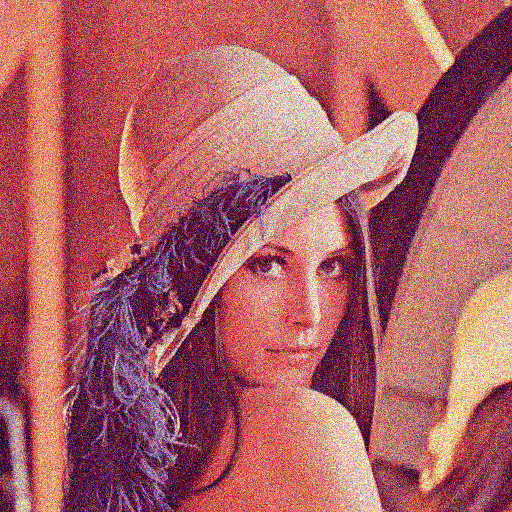
\includegraphics[width=\linewidth]{slide07_pic02.png}\\
    \small 高斯噪声示例
  \end{minipage}
  \hfill
  \begin{minipage}{0.31\linewidth}
    \centering
    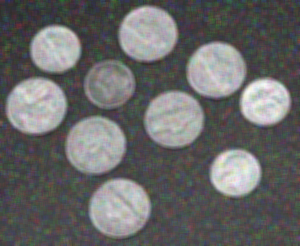
\includegraphics[width=\linewidth]{slide22_pic03.png}\\
    \small 椒盐噪声示例
  \end{minipage}
  \hfill
  \begin{minipage}{0.31\linewidth}
    \centering
    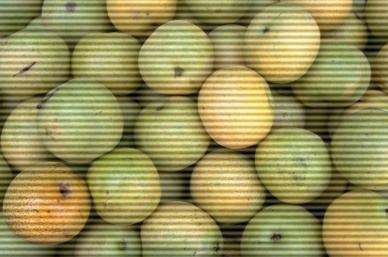
\includegraphics[width=\linewidth]{slide23_pic02.jpg}\\
    \small 周期噪声示例
  \end{minipage}
  \caption{不同噪声模型在图像中的表现。}
  \label{fig:noise-examples}
\end{figure}

\section{空域滤波方法}

\subsection{均值滤波}

均值滤波用邻域平均值替代中心像素：
\begin{equation}
\hat I(x,y)=\frac{1}{|\Omega|}\sum_{(i,j)\in\Omega}I(x+i,y+j),
\end{equation}
其中 $\Omega$ 为 $k\times k$ 滤波窗口。均值滤波相当于低通平滑操作，对零均值随机噪声具有抑制作用，但会同时削弱边缘和纹理。窗口越大，去噪越强，模糊越明显。

\subsection{中值滤波}

中值滤波用邻域中位数替代中心像素：
\begin{equation}
\hat I(x,y)=\operatorname{median}\{I(x+i,y+j)\mid (i,j)\in\Omega\}.
\end{equation}
由于中位数对极端值不敏感，中值滤波特别适合处理椒盐噪声。对于细线、角点和小纹理，过大的窗口仍会造成结构损失，因此实际演示中通常先从 $3\times 3$ 或 $5\times 5$ 开始调整。

\begin{lstlisting}[language=Python,caption={空域滤波模块实现}]
def mean_filter(image: np.ndarray, size: int) -> np.ndarray:
    size = max(1, int(size))
    if image.ndim == 3:
        result = np.stack([
            ndimage.uniform_filter(image[..., channel], size=size)
            for channel in range(image.shape[-1])
        ], axis=-1)
    else:
        result = ndimage.uniform_filter(image, size=size)
    return np.clip(result, 0.0, 1.0)

def median_filter(image: np.ndarray, size: int) -> np.ndarray:
    size = max(1, int(size))
    if image.ndim == 3:
        result = np.stack([
            ndimage.median_filter(image[..., channel], size=size)
            for channel in range(image.shape[-1])
        ], axis=-1)
    else:
        result = ndimage.median_filter(image, size=size)
    return np.clip(result, 0.0, 1.0)
\end{lstlisting}

\begin{figure}[H]
  \centering
  \begin{minipage}{0.30\linewidth}
    \centering
    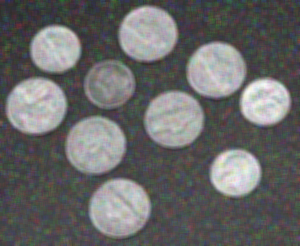
\includegraphics[width=\linewidth]{slide22_pic03.png}\\
    \small 含椒盐噪声
  \end{minipage}
  \hfill
  \begin{minipage}{0.30\linewidth}
    \centering
    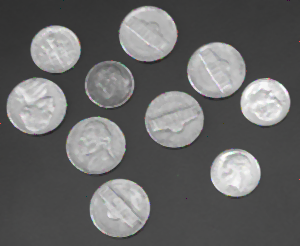
\includegraphics[width=\linewidth]{slide22_pic04.png}\\
    \small 中值滤波
  \end{minipage}
  \hfill
  \begin{minipage}{0.30\linewidth}
    \centering
    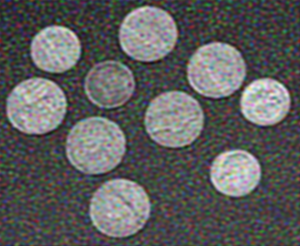
\includegraphics[width=\linewidth]{slide22_pic05.png}\\
    \small 均值滤波
  \end{minipage}
  \caption{椒盐噪声场景下，中值滤波比均值滤波更能抑制孤立脉冲点。}
  \label{fig:salt-pepper}
\end{figure}

\section{频域分析与滤波器设计}

\subsection{二维 DFT 与频谱观察}

对灰度图像 $f(x,y)$，二维离散傅里叶变换为
\begin{equation}
F(u,v)=\sum_{x=0}^{M-1}\sum_{y=0}^{N-1}
f(x,y)e^{-j2\pi(\frac{ux}{M}+\frac{vy}{N})}.
\end{equation}
系统使用 \texttt{fftshift} 将低频移动到频谱中心，并显示 $\log(1+|F(u,v)|)$ 的归一化幅度谱。对于周期噪声，频谱中远离中心的亮点或亮斑往往比原图更容易定位。系统还提供沿 $x$ 轴和 $y$ 轴的一维频谱剖面，计算方式与常见 MATLAB 写法一致：分别沿图像每一行和每一列做 FFT，再取中心行或中心列的幅度谱。

\begin{figure}[H]
  \centering
  \begin{minipage}{0.32\linewidth}
    \centering
    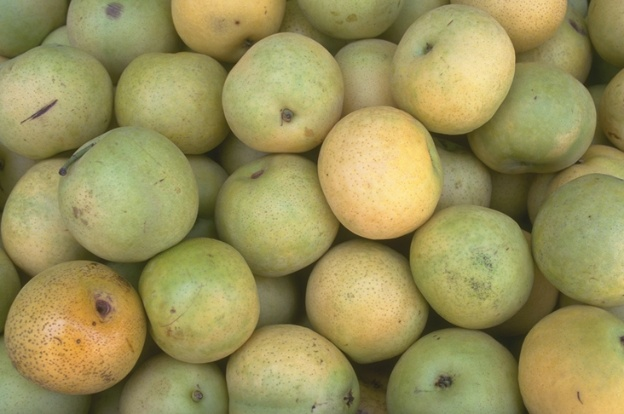
\includegraphics[width=\linewidth]{slide09_pic02.jpg}\\
    \small 原图
  \end{minipage}
  \hfill
  \begin{minipage}{0.32\linewidth}
    \centering
    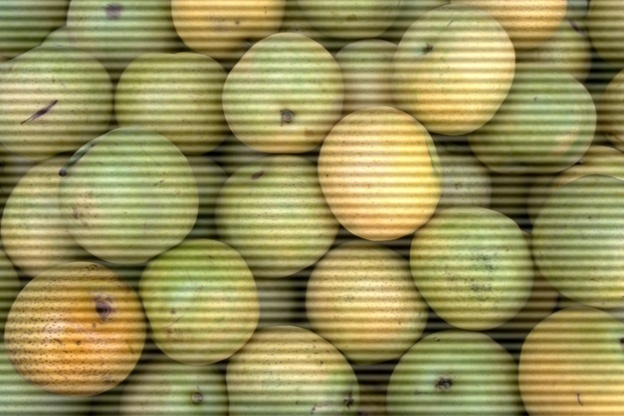
\includegraphics[width=\linewidth]{slide09_pic03.jpg}\\
    \small 含噪图频谱
  \end{minipage}
  \hfill
  \begin{minipage}{0.32\linewidth}
    \centering
    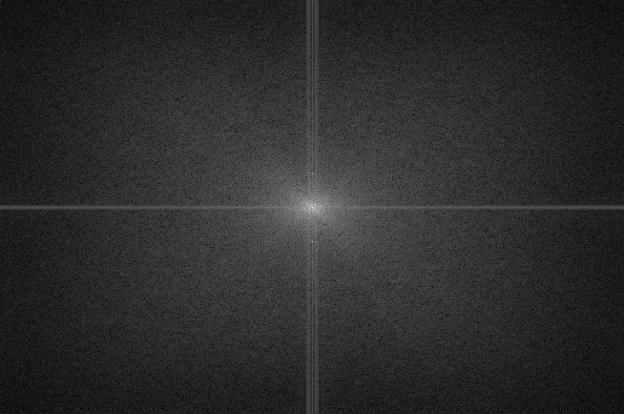
\includegraphics[width=\linewidth]{slide09_pic04.jpg}\\
    \small 频域分布观察
  \end{minipage}
  \caption{通过 DFT 幅度谱观察噪声能量分布。}
  \label{fig:dft}
\end{figure}

\subsection{低通滤波器}

对高斯噪声这类宽带随机扰动，可以先采用低通滤波作为基线。

高斯低通响应为
\begin{equation}
H(u,v)=\exp\left(-\frac{D(u,v)^2}{2D_0^2}\right),
\end{equation}
其中 $D(u,v)$ 是频率点到中心的距离，$D_0$ 为截止半径。高斯低通过渡平滑，振铃较少。

巴特沃斯低通响应为
\begin{equation}
H(u,v)=\frac{1}{1+\left(\frac{D(u,v)}{D_0}\right)^{2n}},
\end{equation}
其中 $n$ 是阶数。阶数越高，过渡带越陡，抑制更强，但也可能带来振铃和边缘伪影。

\subsection{径向 Band-Stop 滤波器}

当异常能量呈同心圆环或某个半径范围内的频带增强时，使用径向带阻滤波器：
\begin{equation}
H(u,v)=\frac{1}{1+\left(
\frac{D(u,v)W}{|D(u,v)^2-D_c^2|}
\right)^{2n}},
\end{equation}
其中 $D_c$ 为带阻中心半径，$W$ 为带宽，$n$ 为阶数。项目支持多组径向 Band-Stop，最终响应为各组响应乘积，并用抑制强度控制最低保留比例。

\subsection{成对陷波带阻滤波器}

周期噪声最典型的频域表现是关于频谱中心成对出现亮点。设某组异常峰相对中心偏移为 $(u_k,v_k)$，则正负陷波距离为
\begin{equation}
D_k(u,v)=\sqrt{(u-u_k)^2+(v-v_k)^2},
\end{equation}
\begin{equation}
D_{-k}(u,v)=\sqrt{(u+u_k)^2+(v+v_k)^2}.
\end{equation}
巴特沃斯成对陷波带阻响应为
\begin{equation}
H_k(u,v)=
\frac{1}{1+\left(\frac{D_0^2}{D_k(u,v)D_{-k}(u,v)}\right)^n}.
\end{equation}
多组陷波点时，系统使用
\begin{equation}
H(u,v)=\prod_{k=1}^{K}\left[1-\alpha_k(1-H_k(u,v))\right],
\end{equation}
其中 $\alpha_k$ 为抑制强度。用户应根据频谱亮点手动输入多组 $(u_k,v_k)$、陷波半径、阶数和抑制强度，而不是完全依赖自动检测。这样更符合信号处理分析流程：先观察频域异常，再设计对应的带阻滤波器。

\begin{lstlisting}[language=Python,caption={成对陷波带阻滤波器实现摘录}]
def butterworth_notch_reject(shape, notches):
    h, w = shape
    yy, xx = np.mgrid[0:h, 0:w]
    center_u = w / 2
    center_v = h / 2
    response = np.ones(shape, dtype=np.float64)

    for notch in notches:
        du = float(notch.get("u", 0))
        dv = float(notch.get("v", 0))
        radius = max(float(notch.get("radius", 8.0)), 1e-6)
        order = max(1, int(notch.get("order", 2)))
        depth = float(np.clip(notch.get("depth", 0.95), 0.0, 1.0))

        d_positive = np.sqrt((xx-center_u-du)**2 + (yy-center_v-dv)**2)
        d_negative = np.sqrt((xx-center_u+du)**2 + (yy-center_v+dv)**2)
        pair_response = 1.0 / (
            1.0 + (radius * radius / np.maximum(d_positive*d_negative, 1e-12)) ** order
        )
        response *= 1.0 - depth * (1.0 - pair_response)

    return np.clip(response, 0.0, 1.0)
\end{lstlisting}

\begin{figure}[H]
  \centering
  \begin{minipage}{0.32\linewidth}
    \centering
    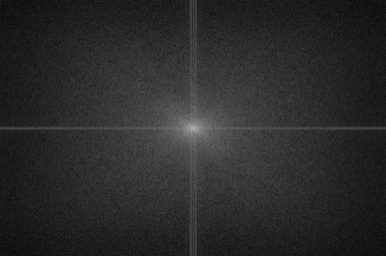
\includegraphics[width=\linewidth]{slide23_pic03.jpg}\\
    \small 含噪图频谱
  \end{minipage}
  \hfill
  \begin{minipage}{0.32\linewidth}
    \centering
    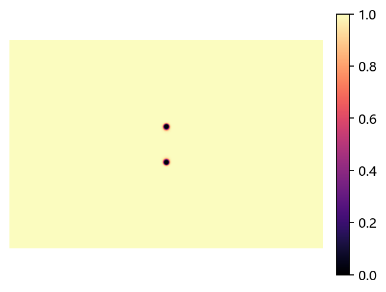
\includegraphics[width=\linewidth]{slide23_pic04.png}\\
    \small 频域响应
  \end{minipage}
  \hfill
  \begin{minipage}{0.32\linewidth}
    \centering
    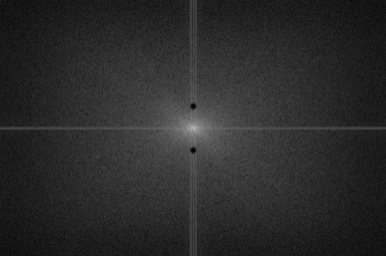
\includegraphics[width=\linewidth]{slide23_pic05.jpg}\\
    \small 滤波后频谱
  \end{minipage}
  \caption{周期噪声的频谱异常与带阻滤波器响应。}
  \label{fig:frequency-response}
\end{figure}

\section{保边滤波与高级去噪}

\subsection{双边滤波}

普通低通滤波只依据空间邻域做平均，因此容易把边缘两侧的像素混合。双边滤波同时考虑空间距离和灰度差异\cite{tomasi1998bilateral}：
\begin{equation}
\hat I(p)=\frac{1}{W_p}\sum_{q\in\Omega}
I(q)
\exp\left(-\frac{\|p-q\|^2}{2\sigma_s^2}\right)
\exp\left(-\frac{\|I(p)-I(q)\|^2}{2\sigma_r^2}\right),
\end{equation}
\begin{equation}
W_p=\sum_{q\in\Omega}
\exp\left(-\frac{\|p-q\|^2}{2\sigma_s^2}\right)
\exp\left(-\frac{\|I(p)-I(q)\|^2}{2\sigma_r^2}\right).
\end{equation}
其中 $\sigma_s$ 控制空间邻域范围，$\sigma_r$ 控制颜色或灰度差异容忍度。$\sigma_r$ 较小时更保边但去噪弱，$\sigma_r$ 较大时平滑更强但可能损失边缘。

\begin{figure}[H]
  \centering
  \begin{minipage}{0.23\linewidth}
    \centering
    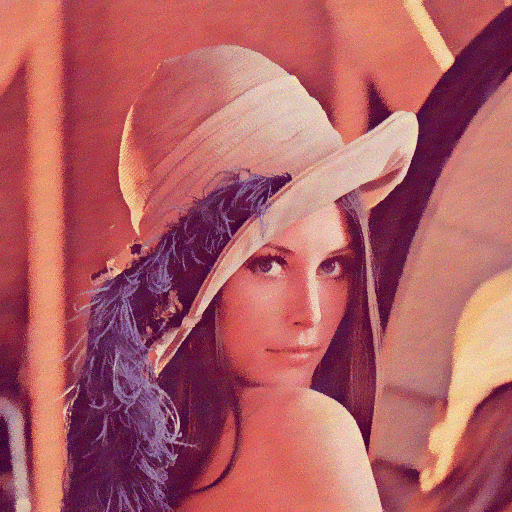
\includegraphics[width=\linewidth]{slide18_pic02.png}\\
    \small 含噪输入
  \end{minipage}
  \hfill
  \begin{minipage}{0.23\linewidth}
    \centering
    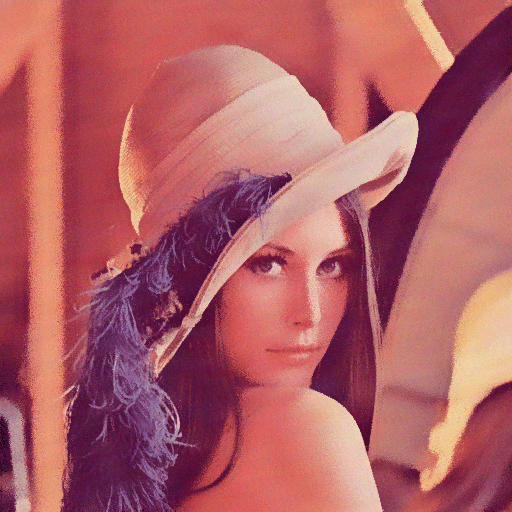
\includegraphics[width=\linewidth]{slide18_pic03.png}\\
    \small 小 $\sigma_r$
  \end{minipage}
  \hfill
  \begin{minipage}{0.23\linewidth}
    \centering
    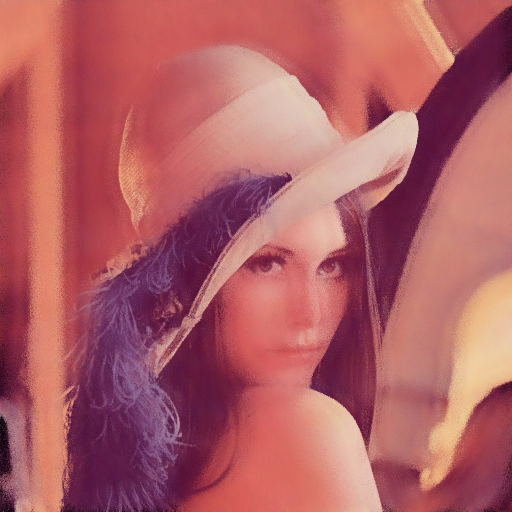
\includegraphics[width=\linewidth]{slide18_pic04.png}\\
    \small 中等 $\sigma_r$
  \end{minipage}
  \hfill
  \begin{minipage}{0.23\linewidth}
    \centering
    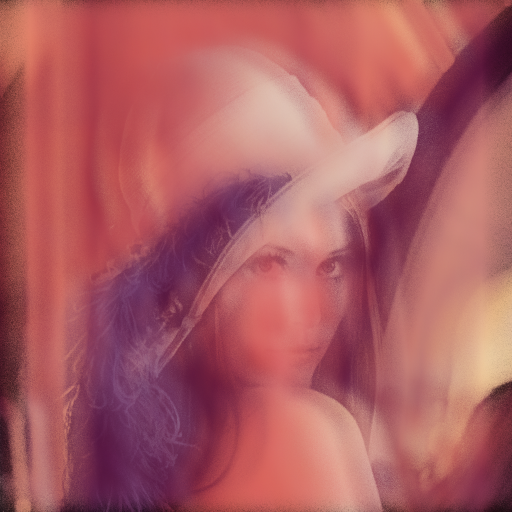
\includegraphics[width=\linewidth]{slide18_pic05.png}\\
    \small 大 $\sigma_r$
  \end{minipage}
  \caption{双边滤波参数对去噪和保边效果的影响。}
  \label{fig:bilateral-params}
\end{figure}

\subsection{非局部均值 NLM}

NLM 不只在局部邻域内平均，而是在较大搜索范围中寻找相似图像块：
\begin{equation}
\hat I(p)=\sum_q w(p,q)I(q),
\end{equation}
\begin{equation}
w(p,q)=\frac{1}{Z_p}\exp\left(-\frac{\|P_p-P_q\|_2^2}{h^2}\right).
\end{equation}
其中 $P_p$ 和 $P_q$ 是以像素 $p,q$ 为中心的小块，$h$ 控制平滑强度，搜索半径控制候选块范围\cite{buades2005nlm}。NLM 的优点是能利用图像内部重复纹理，在保留结构方面通常优于简单均值滤波；缺点是计算量更高，参数过大时也会造成塑料感或细节丢失。

\begin{lstlisting}[language=Python,caption={双边滤波与 NLM 调用实现}]
def bilateral_filter(image, sigma_color, sigma_spatial):
    result = restoration.denoise_bilateral(
        image,
        sigma_color=float(sigma_color),
        sigma_spatial=float(sigma_spatial),
        channel_axis=-1 if image.ndim == 3 else None,
    )
    return np.clip(result, 0.0, 1.0)

def nlm_filter(image, h, patch_size, patch_distance):
    sigma = np.mean(restoration.estimate_sigma(
        image, channel_axis=-1 if image.ndim == 3 else None))
    result = restoration.denoise_nl_means(
        image,
        h=max(float(h) * sigma, 0.01),
        patch_size=int(patch_size),
        patch_distance=int(patch_distance),
        fast_mode=True,
        channel_axis=-1 if image.ndim == 3 else None,
    )
    return np.clip(result, 0.0, 1.0)
\end{lstlisting}

\begin{figure}[H]
  \centering
  \begin{minipage}{0.24\linewidth}
    \centering
    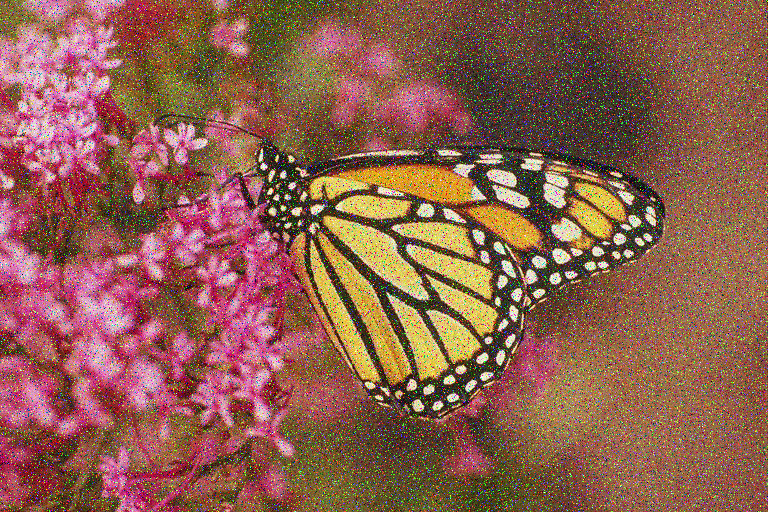
\includegraphics[width=\linewidth]{slide15_pic02.png}\\
    \small 含噪输入
  \end{minipage}
  \hfill
  \begin{minipage}{0.24\linewidth}
    \centering
    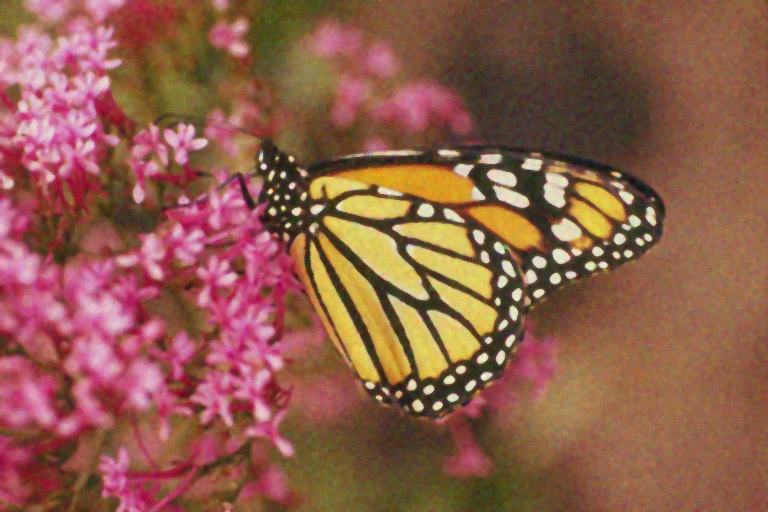
\includegraphics[width=\linewidth]{slide15_pic03.png}\\
    \small 均值滤波
  \end{minipage}
  \hfill
  \begin{minipage}{0.24\linewidth}
    \centering
    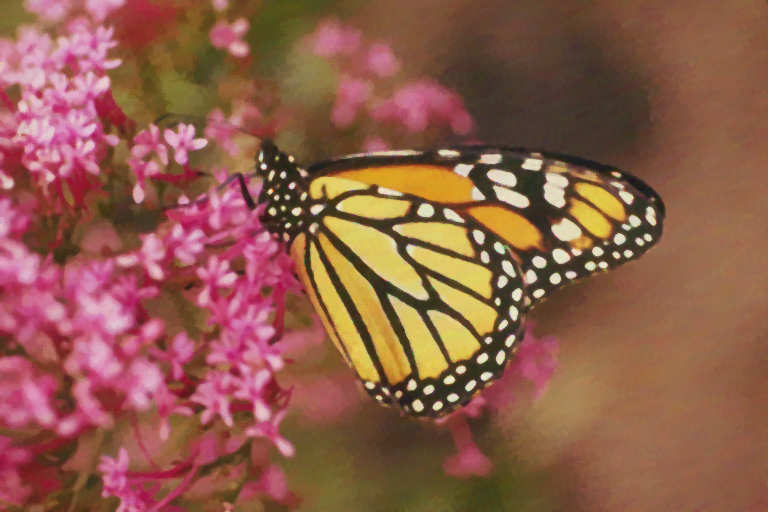
\includegraphics[width=\linewidth]{slide15_pic04.png}\\
    \small 双边滤波
  \end{minipage}
  \hfill
  \begin{minipage}{0.24\linewidth}
    \centering
    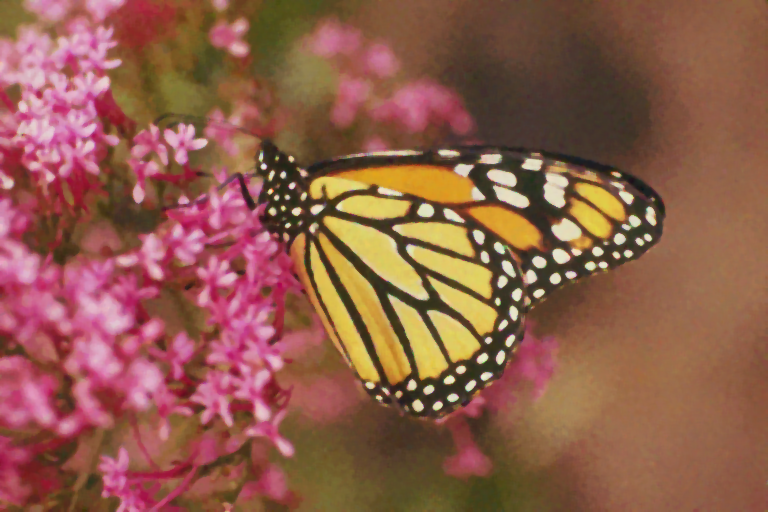
\includegraphics[width=\linewidth]{slide15_pic05.png}\\
    \small NLM
  \end{minipage}
  \caption{均值滤波、双边滤波和 NLM 的视觉效果对比。}
  \label{fig:nlm}
\end{figure}

\section{评价指标与自动调参}

\subsection{有参考图像时的指标}

当用户上传原清晰图，并由程序生成噪声时，原图可作为参考图。系统计算 MSE、PSNR 和 SSIM，其中 SSIM 是经典的结构相似性评价指标\cite{wang2004ssim}：
\begin{equation}
\operatorname{MSE}(I,\hat I)=
\frac{1}{MNC}\sum_{x=1}^{M}\sum_{y=1}^{N}\sum_{c=1}^{C}
(I(x,y,c)-\hat I(x,y,c))^2,
\end{equation}
\begin{equation}
\operatorname{PSNR}=10\log_{10}\frac{L^2}{\operatorname{MSE}},
\end{equation}
\begin{equation}
\operatorname{SSIM}(x,y)=
\frac{(2\mu_x\mu_y+C_1)(2\sigma_{xy}+C_2)}
{(\mu_x^2+\mu_y^2+C_1)(\sigma_x^2+\sigma_y^2+C_2)}.
\end{equation}
项目中像素已经归一化，因此 $L=1$。MSE 越小越好，PSNR 越大越好，SSIM 越接近 1 越好。

\subsection{贝叶斯优化目标函数}

参考图已知时，BO 直接在原尺寸图像上搜索参数，目标分数为
\begin{equation}
J=\operatorname{SSIM}+\frac{\operatorname{PSNR}}{60}
-\min(25\operatorname{MSE},2).
\end{equation}
该分数同时鼓励结构相似、较高信噪比和较低像素误差。均值滤波和中值滤波的核大小只有少量离散奇数候选值，系统会完整评估 $\{1,3,5,7,9,11,13,15\}$，避免随机采样漏掉真正最优核。连续参数较多的方法则使用高斯过程和期望改进选择下一组参数。

当上传图像本身已经含噪、没有清晰参考图时，系统无法计算 MSE、PSNR 和 SSIM。此时程序使用 NIQE-like 无参考质量分数，先计算均值减除对比度归一化系数
\begin{equation}
\operatorname{MSCN}(x,y)=\frac{I(x,y)-\mu(x,y)}{\sigma(x,y)+\epsilon},
\end{equation}
再由偏度、峰度、高频梯度和对比度构造
\begin{equation}
Q_{\text{NR}}=
|\operatorname{skew}(\operatorname{MSCN})|
+|\operatorname{kurtosis}(\operatorname{MSCN})-3|
+\frac{0.08}{G+\epsilon}
+\frac{0.02}{C+\epsilon}.
\end{equation}
无参考场景中 BO 最大化 $-Q_{\text{NR}}$。这类指标只能作为建议，因此系统会把建议参数填入控件，但不锁定用户手动调整。

\begin{lstlisting}[language=Python,caption={自动调参目标分数与离散核搜索}]
def _score(reference, output):
    if reference is None:
        quality = niqe_like_quality(output)
        return -quality.niqe_like, None, None, None, quality.niqe_like

    metrics = reference_metrics(reference, output)
    psnr = 60.0 if np.isinf(metrics.psnr) else metrics.psnr
    mse_penalty = min(metrics.mse * 25.0, 2.0)
    score = float(metrics.ssim + psnr / 60.0 - mse_penalty)
    return score, metrics.mse, metrics.psnr, metrics.ssim, None

def _tune_mean(reference, noisy, iterations, rng):
    candidates = [1, 3, 5, 7, 9, 11, 13, 15]
    best_score = -np.inf
    for size in candidates:
        output = mean_filter(noisy, size)
        score, mse, psnr, ssim, niqe_like = _score(reference, output)
        if score > best_score:
            best_score = score
            best_payload = {"mean_size": size, "_output": output}
    return best_payload, best_score
\end{lstlisting}

\begin{figure}[H]
  \centering
  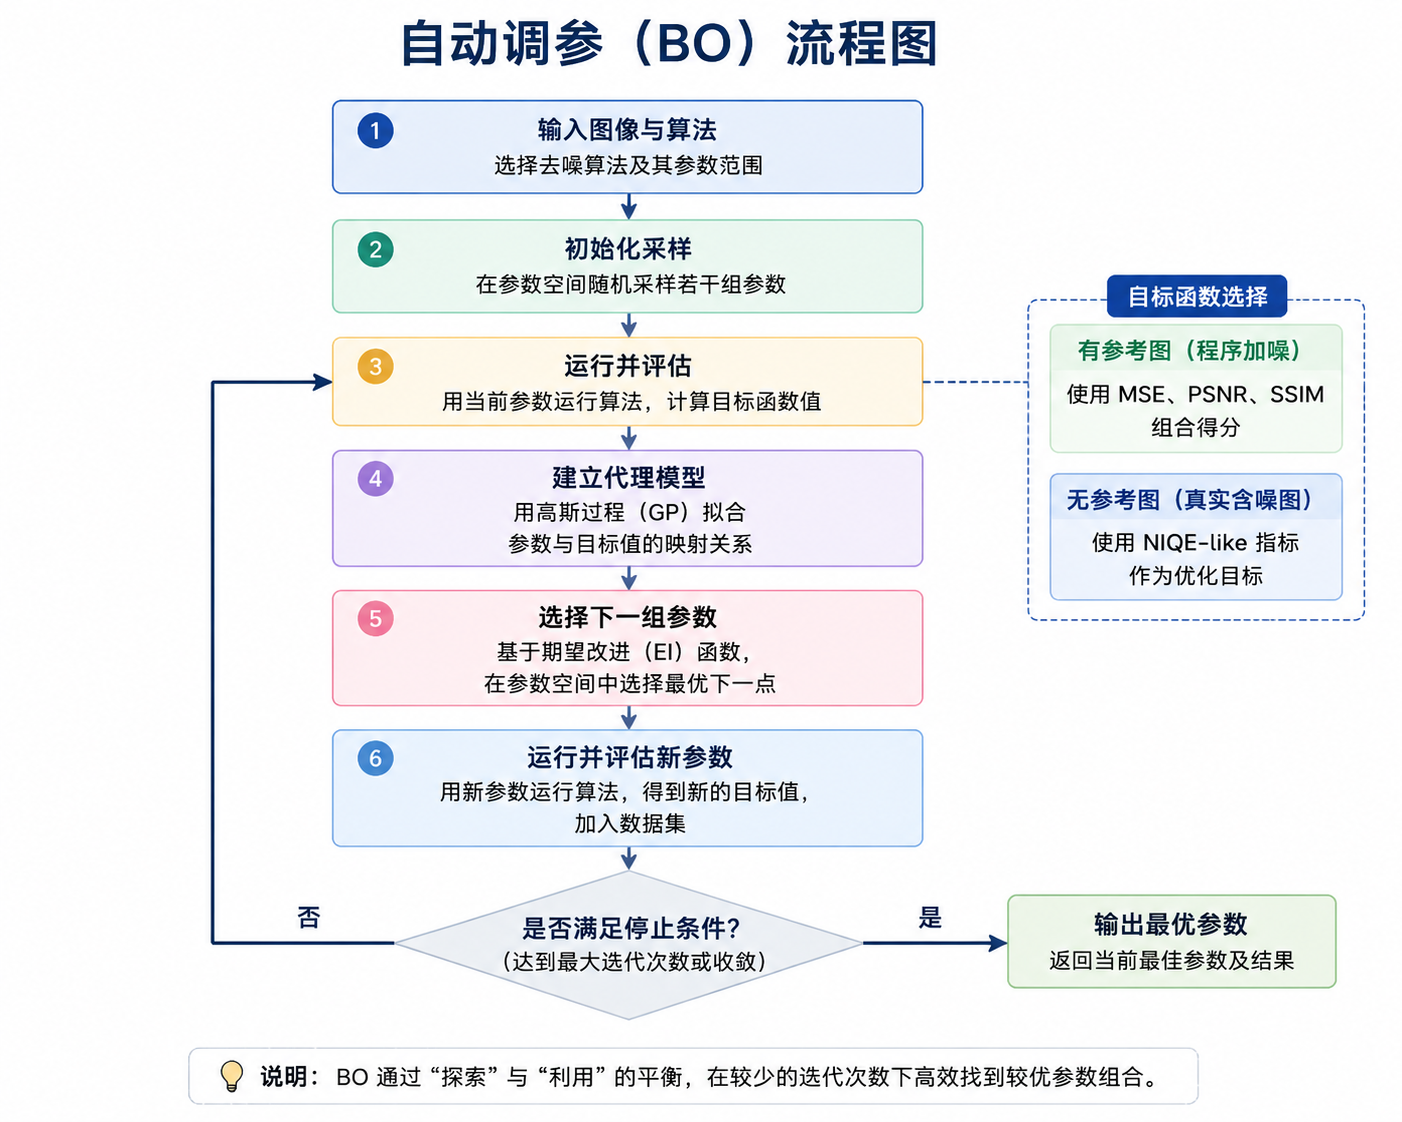
\includegraphics[width=0.80\linewidth]{slide19_pic07.png}
  \caption{BO 调参结果展示：系统给出最佳参数、指标和搜索摘要。}
  \label{fig:bo}
\end{figure}

\section{后处理锐化}

去噪算法本质上会抑制高频成分，因此部分结果会出现发糊现象。系统增加“后处理锐化”导航页，用户可以从当前滤波方法输出中手动选择一张图，再点击按钮执行 USM 非锐化掩膜：
\begin{equation}
B=G_{\sigma}*I,
\end{equation}
\begin{equation}
M=I-B,
\end{equation}
\begin{equation}
I_s=\operatorname{clip}(I+\alpha M,0,1).
\end{equation}
其中 $B$ 是高斯模糊图，$M$ 是细节掩膜，$\alpha$ 为锐化强度。阈值参数用于抑制幅度较小的细节掩膜，避免把残余噪声一起增强。该过程不是自动执行，而是作为滤波后的人工后处理步骤。

\begin{lstlisting}[language=Python,caption={USM 非锐化掩膜实现}]
def unsharp_mask(image, radius, amount, threshold=0.0):
    image = np.clip(image, 0.0, 1.0)
    sigma = max(float(radius), 0.1)
    strength = max(float(amount), 0.0)

    if image.ndim == 3:
        blurred = np.stack([
            ndimage.gaussian_filter(image[..., channel], sigma=sigma)
            for channel in range(image.shape[-1])
        ], axis=-1)
    else:
        blurred = ndimage.gaussian_filter(image, sigma=sigma)

    detail = image - blurred
    if threshold > 0:
        detail = np.where(np.abs(detail) >= threshold, detail, 0.0)
    return np.clip(image + strength * detail, 0.0, 1.0)
\end{lstlisting}

\begin{figure}[H]
  \centering
  \begin{minipage}{0.42\linewidth}
    \centering
    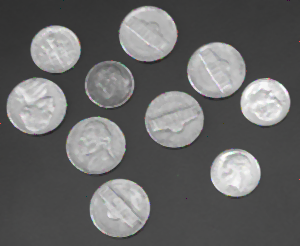
\includegraphics[width=\linewidth]{new_image/中值滤波.png}\\
    \small 滤波后图像
  \end{minipage}
  \hfill
  \begin{minipage}{0.42\linewidth}
    \centering
    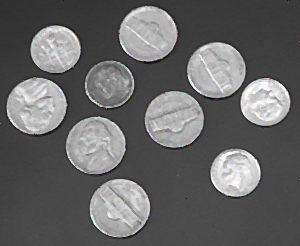
\includegraphics[width=\linewidth]{new_image/usm_sharpened.png}\\
    \small USM 锐化后
  \end{minipage}
  \caption{USM 后处理用于增强滤波后被削弱的细节。}
  \label{fig:sharpen}
\end{figure}

\section{实验结果与分析}

\subsection{高斯噪声实验}

在高斯噪声场景中，均值滤波可以降低随机起伏，但边缘和纹理容易被一起平滑；双边滤波在平坦区域有较好降噪效果，并能通过灰度相似性约束减少跨边缘平均；NLM 在图像存在重复纹理时通常能保留更多细节。频域低通在高频噪声明显时有效，但截止半径过小会造成整体模糊。

\begin{figure}[H]
  \centering
  \begin{minipage}{0.23\linewidth}
    \centering
    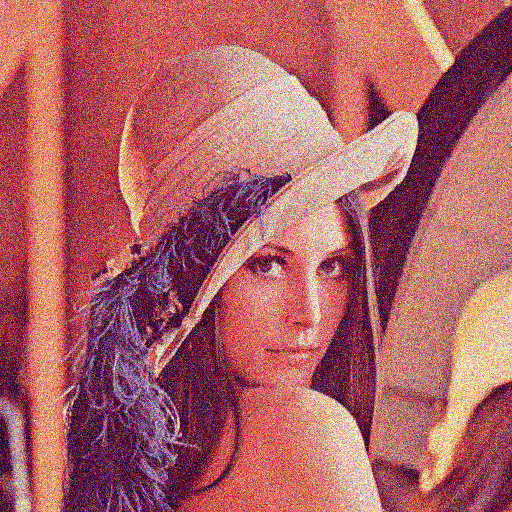
\includegraphics[width=\linewidth]{slide21_pic02.png}\\
    \small 含噪图
  \end{minipage}
  \hfill
  \begin{minipage}{0.23\linewidth}
    \centering
    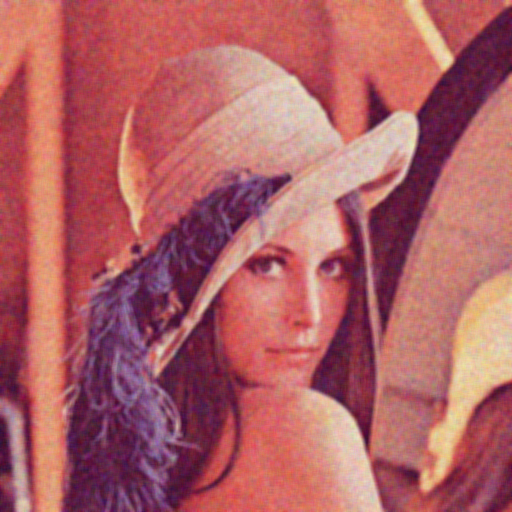
\includegraphics[width=\linewidth]{slide21_pic03.png}\\
    \small 均值滤波
  \end{minipage}
  \hfill
  \begin{minipage}{0.23\linewidth}
    \centering
    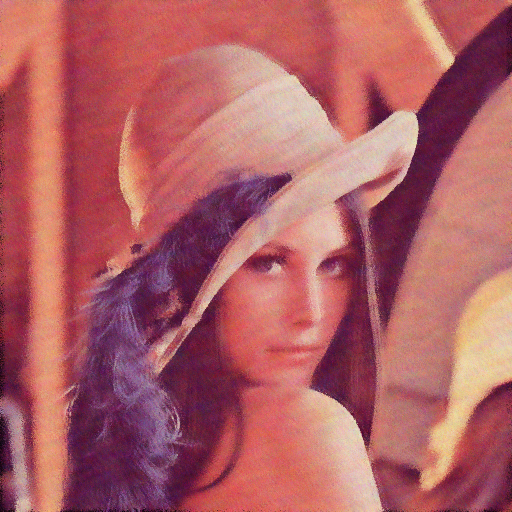
\includegraphics[width=\linewidth]{slide21_pic04.png}\\
    \small 双边滤波
  \end{minipage}
  \hfill
  \begin{minipage}{0.23\linewidth}
    \centering
    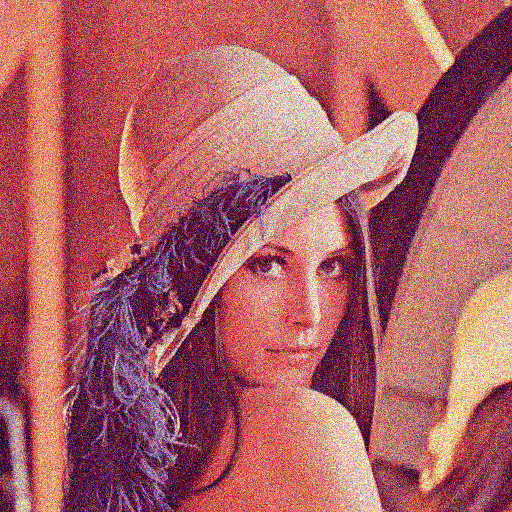
\includegraphics[width=\linewidth]{slide21_pic05.png}\\
    \small NLM
  \end{minipage}
  \caption{高斯噪声实验中不同滤波方法的效果对比。}
  \label{fig:gaussian-exp}
\end{figure}

\subsection{椒盐噪声实验}

椒盐噪声的主要特点是像素出现极端值。均值滤波会把这些极端值扩散到邻域，导致局部灰斑；中值滤波通过排序选择中位数，能有效移除孤立黑白点。因此在椒盐噪声下，中值滤波通常是最直接有效的基线方法。

\begin{figure}[H]
  \centering
  \begin{minipage}{0.42\linewidth}
    \centering
    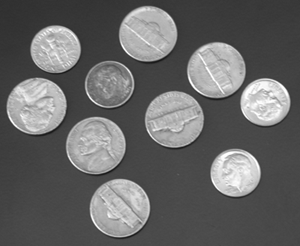
\includegraphics[width=\linewidth]{new_image/coins.png}\\
    \small 原图
  \end{minipage}
  \hfill
  \begin{minipage}{0.42\linewidth}
    \centering
    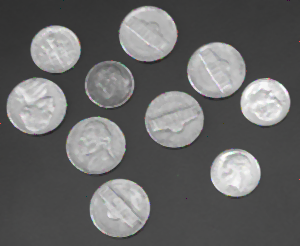
\includegraphics[width=\linewidth]{new_image/中值滤波.png}\\
    \small 中值滤波结果
  \end{minipage}
  \caption{硬币图像的中值滤波实验结果。}
  \label{fig:median-coins-exp}
\end{figure}

\subsection{周期噪声实验}

周期噪声在空域中表现为规则条纹，在频域中表现为关于中心成对出现的离散亮点或亮斑。实验时，应先观察含噪图频谱和 $x/y$ 轴频谱剖面，定位异常峰相对中心的偏移，再设置一组或多组陷波点。若异常能量呈环状或径向频带分布，则使用多组径向 Band-Stop。

\begin{figure}[H]
  \centering
  \begin{minipage}{0.47\linewidth}
    \centering
    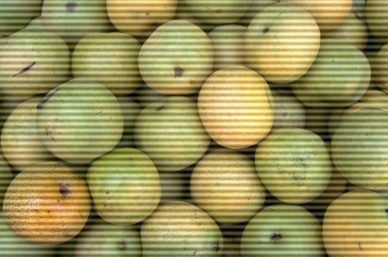
\includegraphics[width=\linewidth]{new_image/含噪图2.png}\\
    \small 含噪图
  \end{minipage}
  \hfill
  \begin{minipage}{0.47\linewidth}
    \centering
    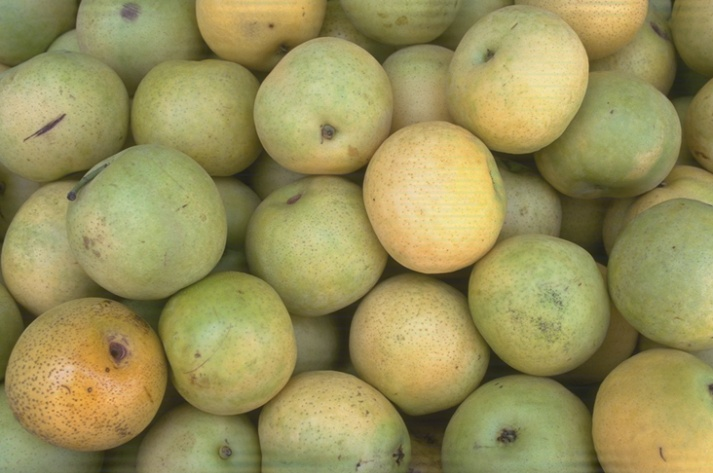
\includegraphics[width=\linewidth]{new_image/去噪结果图.png}\\
    \small 频域滤波结果
  \end{minipage}
  \caption{周期噪声场景下的频域滤波前后对比。}
  \label{fig:periodic-exp}
\end{figure}

\subsection{混合噪声实验}

混合噪声同时包含连续型随机扰动和离散脉冲点，直接使用单一滤波器往往效果不稳定。若只使用均值滤波，高斯成分会被平滑，但椒盐点会被扩散为局部灰斑；若只使用中值滤波，脉冲点会被有效移除，但连续高斯噪声仍然会残留在平坦区域。因此本项目在混合噪声场景中提供“中值预处理”选项：先用小窗口中值滤波去除脉冲点，再把预处理结果交给均值滤波、频域滤波、双边滤波或 NLM。

从信号处理角度看，这相当于把不同类型的噪声分阶段处理。椒盐噪声是稀疏强脉冲，优先用非线性排序滤波抑制；高斯噪声分布更连续，可以再用平滑类或保边类滤波降低方差。若直接增大均值核或双边滤波强度，虽然也能压低噪声，但代价通常是边缘变软和纹理丢失。分阶段处理的优势在于每一步只针对一种主要失真，参数更容易解释。

\begin{table}[H]
\centering
\caption{不同噪声场景下的推荐处理策略}
\begin{tabular}{p{0.20\linewidth}p{0.32\linewidth}p{0.34\linewidth}}
\toprule
噪声场景 & 主要频域或空域特征 & 推荐方法 \\
\midrule
高斯噪声 & 全局随机起伏，高频能量整体增强 & 均值滤波、低通滤波、双边滤波、NLM \\
椒盐噪声 & 局部极大或极小脉冲点 & 中值滤波，小窗口优先 \\
周期噪声 & 频谱中心两侧成对亮点或亮斑 & 成对陷波带阻，多组手动配置 \\
混合噪声 & 脉冲点与连续随机扰动共存 & 中值预处理，再使用保边或频域方法 \\
\bottomrule
\end{tabular}
\end{table}

混合噪声实验说明“算法组合”并不是简单堆叠。合理组合应当建立在噪声模型分析基础上：先判断噪声是否存在稀疏极端点，再判断是否存在周期性结构，最后选择平滑或保边策略处理剩余随机扰动。这样可以把课程中的系统思想体现出来，即复杂系统可以分解为多个针对性更强的子系统。

\subsection{边缘与灰度直方图观察}

仅凭肉眼观察滤波结果容易受到显示尺寸、屏幕亮度和颜色偏差影响，因此系统额外提供边缘图和灰度直方图两个辅助视图。边缘图使用 Canny 思路提取结构轮廓，用于观察滤波后边缘是否断裂、变粗或消失。灰度直方图统计图像灰度分布，用于观察噪声是否导致分布变宽、双峰是否被抹平、椒盐噪声是否在 0 和 1 附近形成异常峰。

边缘保留观察尤其适合比较均值滤波、双边滤波和 NLM。均值滤波的边缘图通常更稀疏，说明部分细节被平滑掉；双边滤波在物体边界处能保留较连续的轮廓，但参数过大时仍会削弱细线；NLM 若参数合适，能在保留纹理的同时降低随机噪声，但计算开销较高。直方图则可以补充说明：过强平滑会使灰度分布向中间集中，而锐化可能重新拉开局部对比度。

\begin{lstlisting}[language=Python,caption={边缘图和灰度直方图分析实现}]
def edge_map(image: np.ndarray) -> np.ndarray:
    gray = to_gray(image)
    return feature.canny(
        filters.gaussian(gray, sigma=0.6),
        sigma=1.0
    ).astype(float)

def histogram(image: np.ndarray, bins: int = 64):
    gray = to_gray(image)
    values, edges = np.histogram(
        gray.ravel(), bins=bins, range=(0.0, 1.0), density=True
    )
    centers = (edges[:-1] + edges[1:]) / 2.0
    return centers, values
\end{lstlisting}

这些观察视图不会替代 MSE、PSNR 和 SSIM，但能解释指标背后的视觉原因。例如某个方法 PSNR 较高但边缘图明显稀疏，说明它可能通过过度平滑降低了像素误差；某个方法 SSIM 较高但直方图对比度降低，说明结构保持较好但视觉锐度可能不足。因此系统中同时呈现图像、频谱、边缘、直方图和指标，能够更完整地评价去噪方法。

\section{参数选择讨论}

\subsection{空域参数}

均值滤波和中值滤波的关键参数都是核大小。核越大，平滑越强，但图像边缘和细节损失越明显。对于弱高斯噪声，$3\times3$ 或 $5\times5$ 均值滤波可作为起点；对于椒盐噪声，$3\times3$ 中值滤波通常先验更合理。混合噪声中可先用小窗口中值滤波移除脉冲点，再将结果送入其他滤波器。

\subsection{频域参数}

频域滤波参数必须和频谱观察结合。低通滤波的截止半径控制保留的低频范围，半径过小会丢失边缘。径向 Band-Stop 的中心半径和带宽应对应异常环带位置。成对陷波带阻的 $(u_k,v_k)$ 应来自频谱中相对中心的亮点偏移，陷波半径控制抑制范围，阶数控制过渡陡峭程度，抑制强度控制最低保留比例。

\subsection{保边与 NLM 参数}

双边滤波的 $\sigma_s$ 较大时会扩大空间平滑范围，$\sigma_r$ 较大时会放宽颜色差异约束。若 $\sigma_r$ 过小，边缘保留较强但噪声去除有限；若 $\sigma_r$ 过大，算法退化为更强的平滑，边缘会变软。因此演示时通常先固定 $\sigma_s$，逐步增大 $\sigma_r$，观察平坦区域噪声下降与边缘变软之间的折中。

NLM 的主要参数包括平滑强度 $h$、图像块大小和搜索距离。$h$ 越大，相似块的加权平均越强，随机噪声下降更明显，但纹理可能被合并成块状或塑料感；$h$ 过小时，算法会过于保守，噪声残留较多。图像块大小决定相似性比较的局部结构尺度，较小块适合细纹理和边缘丰富的图像，较大块更适合结构重复且噪声较强的场景。搜索距离决定候选块范围，范围越大越可能找到相似块，但计算量明显上升。实际调参时可先使用 $5\times5$ 或 $7\times7$ 图像块、中等搜索距离，再根据纹理保留情况调整 $h$。

\section{系统特点与不足}

\subsection{系统特点}

本项目的主要特点包括：
\begin{enumerate}
  \item 实时性：上传图像后立即按当前参数计算，不依赖预处理好的固定图片。
  \item 可解释性：同时展示图像、频谱、响应、直方图、边缘和指标，使滤波设计与结果变化可以对应起来。
  \item 参数完整性：所有关键参数均可手动输入，适合课堂现场按频谱亮点精确设置陷波点。
  \item 方法覆盖面：覆盖空域、频域、保边、高级去噪和后处理锐化。
  \item 可复现性：支持当前参数 JSON、图片和 CSV 的一键导出。
\end{enumerate}

\subsection{不足与改进方向}

系统仍有进一步改进空间。首先，频域异常检测只能给出候选建议，复杂真实图像中纹理本身也会形成亮线或亮点，仍需要人工判断。其次，NLM 和 BO 搜索计算量较高，面对大图像时需要在实时性和质量之间折中。再次，NIQE-like 指标只是轻量无参考指标，不能完全代表主观视觉质量。后续可以引入更标准的无参考图像质量评价模型，或增加小波阈值、BM3D、深度学习去噪等方法作为扩展对比。

\section*{成员分工}
\addcontentsline{toc}{section}{成员分工}

\begin{table}[H]
\centering
\caption{成员分工}
\begin{tabular}{lll}
\toprule
成员 & 主要工作 & 工作量 \\
\midrule
智文静 & 负责课堂答辩与展示与报告 & 25\% \\
奚奕萱 & 负责 PPT 制作与报告 & 25\% \\
汪语菲 & 负责 PPT 制作与报告 & 25\% \\
黄冠杰 & 负责项目代码与报告 & 25\% \\
\bottomrule
\end{tabular}
\end{table}

\section*{结论}
\addcontentsline{toc}{section}{结论}

本项目完成了一个图像去噪实时演示系统。系统从空域滤波出发，逐步扩展到频域 DFT 分析、低通与带阻响应设计、双边滤波、NLM、自动调参和后处理锐化。通过实时上传和实时计算，演示者可以现场展示不同噪声模型下算法效果的差异，并通过频谱图解释周期噪声为什么适合使用成对陷波带阻滤波器。整体上，本项目既覆盖了信号与系统课程中的滤波和频域分析知识，也形成了功能完整、易于演示和复现实验的交互式程序。

\clearpage
\addcontentsline{toc}{section}{参考文献}
\begin{thebibliography}{99}
\bibitem{gonzalez2018digital}
GONZALEZ R C, WOODS R E. Digital image processing[M]. 4th ed. New York: Pearson, 2018.

\bibitem{tomasi1998bilateral}
TOMASI C, MANDUCHI R. Bilateral filtering for gray and color images[C]//Proceedings of the Sixth International Conference on Computer Vision. Bombay: IEEE, 1998: 839-846.

\bibitem{buades2005nlm}
BUADES A, COLL B, MOREL J M. A non-local algorithm for image denoising[C]//Proceedings of the 2005 IEEE Computer Society Conference on Computer Vision and Pattern Recognition. San Diego: IEEE, 2005: 60-65.

\bibitem{wang2004ssim}
WANG Z, BOVIK A C, SHEIKH H R, et al. Image quality assessment: from error visibility to structural similarity[J]. IEEE Transactions on Image Processing, 2004, 13(4): 600-612.

\bibitem{skimage}
VAN DER WALT S, SCHONBERGER J L, NUNEZ-IGLESIAS J, et al. scikit-image: image processing in Python[J]. PeerJ, 2014, 2: e453.
\end{thebibliography}

\end{document}
